\documentclass[11pt,a4paper,oneside]{book}

% ============================================
% PACKAGES
% ============================================
\usepackage[utf8]{inputenc}
\usepackage[T1]{fontenc}
\usepackage[english]{babel}
\usepackage{geometry}
\usepackage{titlesec}
\usepackage{fancyhdr}
\usepackage{graphicx}
\usepackage{xcolor}
\usepackage{tcolorbox}
\usepackage{tikz}
\usepackage{pgfplots}
\usepackage{listings}
\usepackage{hyperref}
\usepackage{tabularx}
\usepackage{booktabs}
\usepackage{enumitem}
\usepackage{fontawesome5}
\usepackage{multicol}
\usepackage{amsmath}
\usepackage{array}

% ============================================
% DOCUMENT GEOMETRY
% ============================================
\geometry{
    a4paper,
    left=2.5cm,
    right=2.5cm,
    top=2.5cm,
    bottom=3cm,
    headheight=15pt
}

% ============================================
% COLOR DEFINITIONS
% ============================================
\definecolor{primarynavy}{RGB}{20,40,80}
\definecolor{accentteal}{RGB}{0,150,136}
\definecolor{accentorange}{RGB}{255,120,50}
\definecolor{darkgray}{RGB}{50,50,50}
\definecolor{lightgray}{RGB}{240,240,240}
\definecolor{codebackground}{RGB}{245,245,250}
\definecolor{keywordcolor}{RGB}{0,102,204}
\definecolor{stringcolor}{RGB}{163,21,21}

% ============================================
% TIKZ LIBRARIES
% ============================================
\usetikzlibrary{shapes,arrows,positioning,shadows,calc}
\pgfplotsset{compat=1.18}

% ============================================
% HYPERREF SETUP
% ============================================
\hypersetup{
    colorlinks=true,
    linkcolor=primarynavy,
    filecolor=accentteal,
    urlcolor=accentteal,
    citecolor=primarynavy,
    pdftitle={Real Scout - Real Estate Application Documentation},
    pdfauthor={Mausam Kar},
    pdfsubject={Mobile Application Development},
    pdfkeywords={React Native, Real Estate, Mobile App, Appwrite}
}

% ============================================
% CHAPTER & SECTION STYLING
% ============================================
\titleformat{\chapter}[block]
  {\normalfont\huge\bfseries\color{primarynavy}}
  {\colorbox{accentteal}{\parbox{1.5cm}{\centering\textcolor{white}{\fontsize{40}{48}\selectfont\thechapter}}}}
  {1em}
  {\Huge}
  [\vspace{2ex}\titlerule]

\titleformat{\section}
  {\normalfont\Large\bfseries\color{primarynavy}}
  {\thesection}
  {1em}
  {}
  [\vspace{0.5ex}{\color{accentteal}\titlerule[1pt]}]

\titleformat{\subsection}
  {\normalfont\large\bfseries\color{accentteal}}
  {\thesubsection}
  {1em}
  {}

% ============================================
% HEADER & FOOTER
% ============================================
\pagestyle{fancy}
\fancyhf{}
\fancyhead[L]{\nouppercase{\leftmark}}
\fancyhead[R]{\textcolor{accentteal}{\textbf{Real Scout}}}
\fancyfoot[C]{\thepage}
\renewcommand{\headrulewidth}{0.5pt}
\renewcommand{\footrulewidth}{0pt}

% ============================================
% COLORED BOXES
% ============================================
\tcbuselibrary{skins,breakable}

\newtcolorbox{definitionbox}{
    colback=accentteal!5,
    colframe=accentteal,
    fonttitle=\bfseries,
    title=Definition,
    boxrule=1pt,
    arc=3pt,
    breakable
}

\newtcolorbox{keypoint}{
    colback=accentorange!10,
    colframe=accentorange,
    fonttitle=\bfseries,
    title=Key Point,
    boxrule=1pt,
    arc=3pt,
    breakable
}

\newtcolorbox{notebox}{
    colback=primarynavy!5,
    colframe=primarynavy,
    fonttitle=\bfseries,
    title=Note,
    boxrule=1pt,
    arc=3pt,
    breakable
}

% ============================================
% CODE LISTING STYLE
% ============================================
\lstset{
    backgroundcolor=\color{codebackground},
    basicstyle=\ttfamily\small,
    keywordstyle=\color{keywordcolor}\bfseries,
    stringstyle=\color{stringcolor},
    commentstyle=\color{gray}\itshape,
    numberstyle=\tiny\color{gray},
    numbers=left,
    breaklines=true,
    frame=single,
    rulecolor=\color{lightgray},
    tabsize=2,
    captionpos=b,
    showstringspaces=false
}

% ============================================
% DOCUMENT BEGIN
% ============================================
\begin{document}

% ============================================
% TITLE PAGE
% ============================================
\begin{titlepage}
\begin{tikzpicture}[remember picture,overlay]
    % Background gradient
    \fill[primarynavy!90] (current page.south west) rectangle (current page.north east);
    
    % Top accent bar
    \fill[accentteal] (current page.north west) rectangle ([yshift=-3cm]current page.north east);
    
    % Bottom accent bar
    \fill[accentorange] (current page.south west) rectangle ([yshift=2cm]current page.south east);
    
    % Decorative circles
    \foreach \i in {1,...,5}{
        \fill[white,opacity=0.1] ([xshift=\i cm, yshift=-\i cm]current page.north east) circle (2cm);
    }
    
    % Main title box
    \node[text width=12cm,align=center] at (current page.center) {
        {\Huge\bfseries\color{white} REAL SCOUT}\\[1cm]
        {\Large\color{accentorange} Real Estate Mobile Application}\\[0.5cm]
        {\large\color{lightgray} Complete Technical Documentation}\\[3cm]
        {\Large\color{white} A Modern Full-Stack Solution}\\[0.3cm]
        {\large\color{lightgray} React Native • Expo • Appwrite • TypeScript}\\[4cm]
        {\LARGE\bfseries\color{accentteal} Mausam Kar}\\[0.3cm]
        {\large\color{white} Full-Stack Developer \& Mobile Enthusiast}
    };
    
    % Version badge
    \node[fill=accentorange,rounded corners,text=white,font=\bfseries] at ([yshift=3cm]current page.south) {Version 1.0.0 | 2024};
\end{tikzpicture}
\end{titlepage}

\frontmatter

% ============================================
% TABLE OF CONTENTS
% ============================================
\tableofcontents

\mainmatter

% ============================================
% CHAPTER 1: INTRODUCTION
% ============================================
\chapter{Introduction}

\section{Overview}

\textbf{Real Scout} is a modern, full-stack real estate mobile application built with React Native and Expo. It provides users with a seamless experience to browse, search, and explore properties with an intuitive interface and powerful features.

\begin{keypoint}
The application leverages \textbf{Google OAuth} for secure authentication and \textbf{Appwrite} as a backend-as-a-service platform for managing data, authentication, and storage.
\end{keypoint}

\section{Key Highlights}

\begin{itemize}[leftmargin=2cm]
    \item[\faLock] \textbf{Secure Authentication} with Google OAuth 2.0
    \item[\faHome] \textbf{Dynamic Property Listings} with advanced search and filtering
    \item[\faMobile] \textbf{Cross-platform} support (iOS \& Android)
    \item[\faPalette] \textbf{Modern UI/UX} with NativeWind (Tailwind CSS for React Native)
    \item[\faBolt] \textbf{Fast Performance} with optimized data fetching
    \item[\faSync] \textbf{Real-time Updates} with Appwrite
    \item[\faSeedling] \textbf{Database Seeding} utility for quick setup
\end{itemize}

\section{Project Metadata}

\begin{table}[h]
\centering
\begin{tabularx}{\textwidth}{lX}
\toprule
\textbf{Attribute} & \textbf{Details} \\
\midrule
Version & 1.0.0 \\
License & MIT License \\
Platform & iOS \& Android \\
Repository & \url{https://github.com/Mausam5055/Real-Estate-APP} \\
Author & Mausam Kar \\
Status & Production Ready \\
\bottomrule
\end{tabularx}
\caption{Project Metadata}
\end{table}

% ============================================
% CHAPTER 2: FEATURES
% ============================================
\chapter{Features}

\section{Implemented Features}

The following table presents a comprehensive overview of all implemented and planned features:

\begin{table}[h]
\small
\centering
\begin{tabularx}{\textwidth}{>{\bfseries}l X c}
\toprule
\textbf{Feature} & \textbf{Description} & \textbf{Status} \\
\midrule
Google Authentication & Seamless OAuth 2.0 login with Google & \textcolor{green}{\faCheck} \\
Property Browsing & Browse all available properties with pagination & \textcolor{green}{\faCheck} \\
Advanced Search & Search properties by name, address, or type & \textcolor{green}{\faCheck} \\
Smart Filters & Filter properties by type (House, Apartment, Villa) & \textcolor{green}{\faCheck} \\
Property Details & Comprehensive property info with image gallery & \textcolor{green}{\faCheck} \\
User Profiles & Manage user settings and preferences & \textcolor{green}{\faCheck} \\
Agent Information & View detailed agent profiles and contact info & \textcolor{green}{\faCheck} \\
Reviews \& Ratings & Read property reviews and ratings & \textcolor{green}{\faCheck} \\
Facilities Overview & View property amenities (Gym, Pool, Parking) & \textcolor{green}{\faCheck} \\
Database Seeding & Quick setup with sample data & \textcolor{green}{\faCheck} \\
Responsive Design & Optimized for all screen sizes & \textcolor{green}{\faCheck} \\
Offline Support & Cache data for offline viewing & \textcolor{orange}{\faCog} \\
Push Notifications & Get notified about new properties & \textcolor{blue}{\faClock} \\
Favorites/Wishlist & Save properties for later viewing & \textcolor{blue}{\faClock} \\
Property Comparison & Compare multiple properties side-by-side & \textcolor{blue}{\faClock} \\
\bottomrule
\end{tabularx}
\caption{Feature Implementation Status}
\end{table}

\textbf{Legend:} \textcolor{green}{\faCheck} Implemented | \textcolor{orange}{\faCog} In Progress | \textcolor{blue}{\faClock} Planned

% ============================================
% CHAPTER 3: ARCHITECTURE
% ============================================
\chapter{Architecture}

\section{System Architecture}

Real Scout follows a clean, scalable architecture pattern with clear separation of concerns across multiple layers.

\begin{figure}[h]
\centering
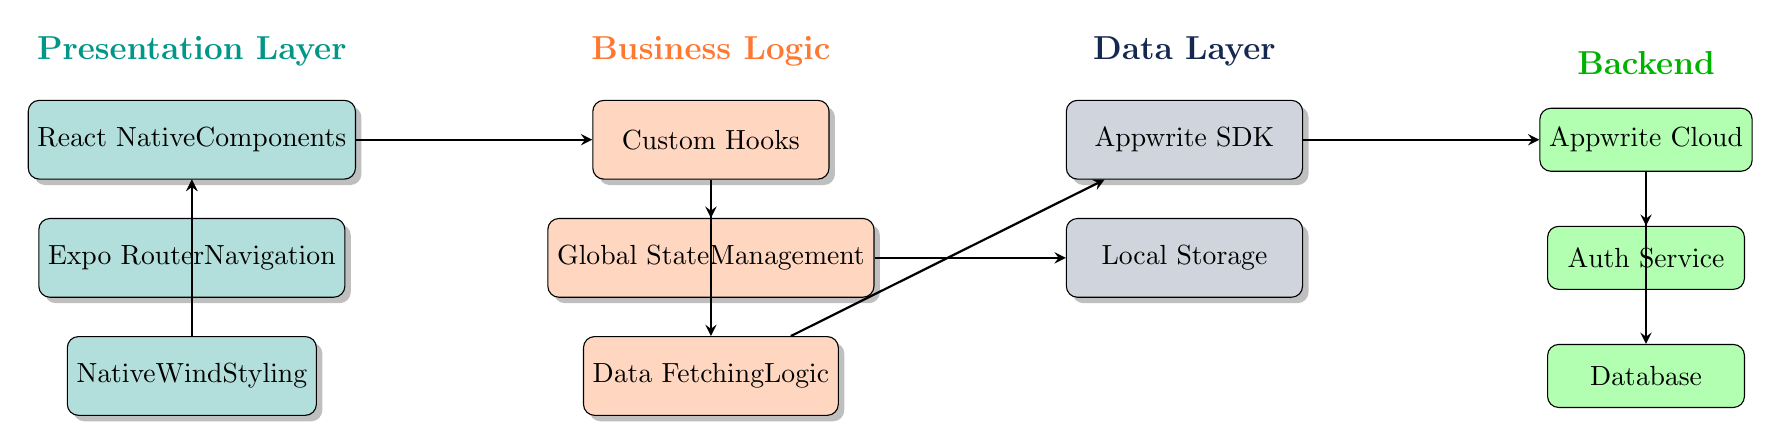
\begin{tikzpicture}[
    node distance=1.5cm,
    box/.style={rectangle, rounded corners, minimum width=3cm, minimum height=1cm, text centered, draw=black, fill=blue!20, drop shadow},
    service/.style={rectangle, rounded corners, minimum width=2.5cm, minimum height=0.8cm, text centered, draw=black, fill=green!20},
    arrow/.style={->, >=stealth, thick}
]

% Presentation Layer
\node[box, fill=accentteal!30] (rn) at (0,0) {React Native\\Components};
\node[box, fill=accentteal!30, below of=rn] (router) {Expo Router\\Navigation};
\node[box, fill=accentteal!30, below of=router] (style) {NativeWind\\Styling};

% Business Logic Layer
\node[box, fill=accentorange!30, right=3cm of rn] (hooks) {Custom Hooks};
\node[box, fill=accentorange!30, below of=hooks] (state) {Global State\\Management};
\node[box, fill=accentorange!30, below of=state] (fetch) {Data Fetching\\Logic};

% Data Layer
\node[box, fill=primarynavy!20, right=3cm of hooks] (sdk) {Appwrite SDK};
\node[box, fill=primarynavy!20, below of=sdk] (storage) {Local Storage};

% Backend Services
\node[service, fill=green!30, right=3cm of sdk] (cloud) {Appwrite Cloud};
\node[service, fill=green!30, below of=cloud] (auth) {Auth Service};
\node[service, fill=green!30, below of=auth] (db) {Database};

% Arrows
\draw[arrow] (rn) -- (hooks);
\draw[arrow] (router) -- (rn);
\draw[arrow] (style) -- (rn);
\draw[arrow] (hooks) -- (state);
\draw[arrow] (hooks) -- (fetch);
\draw[arrow] (fetch) -- (sdk);
\draw[arrow] (state) -- (storage);
\draw[arrow] (sdk) -- (cloud);
\draw[arrow] (cloud) -- (auth);
\draw[arrow] (cloud) -- (db);

% Layer labels
\node[above=0.3cm of rn, font=\bfseries\large, color=accentteal] {Presentation Layer};
\node[above=0.3cm of hooks, font=\bfseries\large, color=accentorange] {Business Logic};
\node[above=0.3cm of sdk, font=\bfseries\large, color=primarynavy] {Data Layer};
\node[above=0.3cm of cloud, font=\bfseries\large, color=green!70!black] {Backend};

\end{tikzpicture}
\caption{System Architecture Diagram}
\end{figure}

\section{Architecture Layers}

\begin{enumerate}
    \item \textbf{Presentation Layer}: React Native components styled with NativeWind providing the user interface
    \item \textbf{Business Logic Layer}: Custom hooks and state management handling application logic
    \item \textbf{Data Layer}: Appwrite SDK integration with local caching for offline support
    \item \textbf{Backend Services}: Appwrite cloud services for authentication, database, and storage
\end{enumerate}

% ============================================
% CHAPTER 4: TECHNOLOGY STACK
% ============================================
\chapter{Technology Stack}

\section{Frontend Technologies}

\begin{table}[h]
\centering
\begin{tabularx}{\textwidth}{l c X}
\toprule
\textbf{Technology} & \textbf{Version} & \textbf{Purpose} \\
\midrule
React Native & 0.81.5 & Cross-platform mobile framework \\
Expo & \textasciitilde{}54.0.0 & Development platform and toolchain \\
TypeScript & \textasciicirc{}5.3.3 & Type-safe JavaScript \\
NativeWind & \textasciicirc{}4.1.23 & Tailwind CSS for React Native \\
Expo Router & \textasciitilde{}6.0.19 & File-based routing \\
React Navigation & \textasciicirc{}7.0.0 & Navigation library \\
\bottomrule
\end{tabularx}
\caption{Frontend Technology Stack}
\end{table}

\section{Backend \& Services}

\begin{table}[h]
\centering
\begin{tabularx}{\textwidth}{l X}
\toprule
\textbf{Technology} & \textbf{Purpose} \\
\midrule
Appwrite & Backend-as-a-Service (BaaS) platform \\
Google OAuth & Authentication provider for secure login \\
Appwrite Databases & NoSQL document database \\
Appwrite Storage & File storage and CDN \\
\bottomrule
\end{tabularx}
\caption{Backend Technology Stack}
\end{table}

\section{Development Tools}

\begin{table}[h]
\centering
\begin{tabularx}{\textwidth}{l X}
\toprule
\textbf{Tool} & \textbf{Purpose} \\
\midrule
Jest & Unit testing framework \\
ESLint & Code linting and quality \\
Babel & JavaScript compiler \\
Metro & JavaScript bundler \\
\bottomrule
\end{tabularx}
\caption{Development Tools}
\end{table}

% ============================================
% CHAPTER 5: AUTHENTICATION
% ============================================
\chapter{Authentication}

\section{Authentication Flow}

The application uses Google OAuth 2.0 for secure user authentication. The following sequence diagram illustrates the complete authentication process:

\begin{figure}[h]
\centering
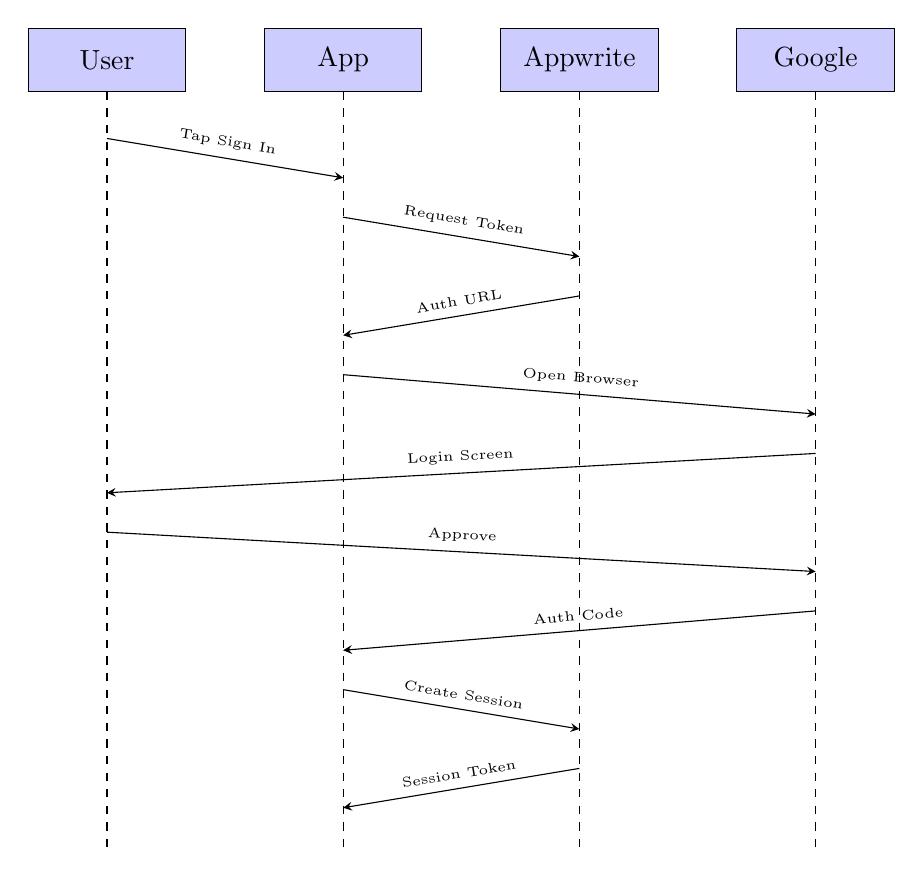
\begin{tikzpicture}[
    entity/.style={rectangle, minimum width=2cm, minimum height=0.8cm, text centered, draw=black, fill=blue!20},
    message/.style={->, >=stealth}
]

% Entities
\node[entity] (user) at (0,0) {User};
\node[entity] (app) at (3,0) {App};
\node[entity] (appwrite) at (6,0) {Appwrite};
\node[entity] (google) at (9,0) {Google};

% Lifelines
\draw[dashed] (user) -- (0,-10);
\draw[dashed] (app) -- (3,-10);
\draw[dashed] (appwrite) -- (6,-10);
\draw[dashed] (google) -- (9,-10);

% Messages
\draw[message] (0,-1) -- node[above, sloped, font=\tiny] {Tap Sign In} (3,-1.5);
\draw[message] (3,-2) -- node[above, sloped, font=\tiny] {Request Token} (6,-2.5);
\draw[message] (6,-3) -- node[above, sloped, font=\tiny] {Auth URL} (3,-3.5);
\draw[message] (3,-4) -- node[above, sloped, font=\tiny] {Open Browser} (9,-4.5);
\draw[message] (9,-5) -- node[above, sloped, font=\tiny] {Login Screen} (0,-5.5);
\draw[message] (0,-6) -- node[above, sloped, font=\tiny] {Approve} (9,-6.5);
\draw[message] (9,-7) -- node[above, sloped, font=\tiny] {Auth Code} (3,-7.5);
\draw[message] (3,-8) -- node[above, sloped, font=\tiny] {Create Session} (6,-8.5);
\draw[message] (6,-9) -- node[above, sloped, font=\tiny] {Session Token} (3,-9.5);

\end{tikzpicture}
\caption{OAuth 2.0 Authentication Sequence}
\end{figure}

\section{Implementation Code}

\begin{lstlisting}[language=JavaScript, caption=Authentication Implementation]
// lib/appwrite.ts
export async function login() {
  const redirectUri = Linking.createURL("/");
  const response = await account.createOAuth2Token(
    OAuthProvider.Google,
    redirectUri
  );

  const browserResult = await openAuthSessionAsync(
    response.toString(),
    redirectUri
  );

  const url = new URL(browserResult.url);
  const secret = url.searchParams.get("secret");
  const userId = url.searchParams.get("userId");

  const session = await account.createSession(userId, secret);
  return session;
}
\end{lstlisting}

% ============================================
% CHAPTER 6: DATABASE SCHEMA
% ============================================
\chapter{Database Schema}

\section{Entity Relationship Diagram}

\begin{figure}[h]
\centering
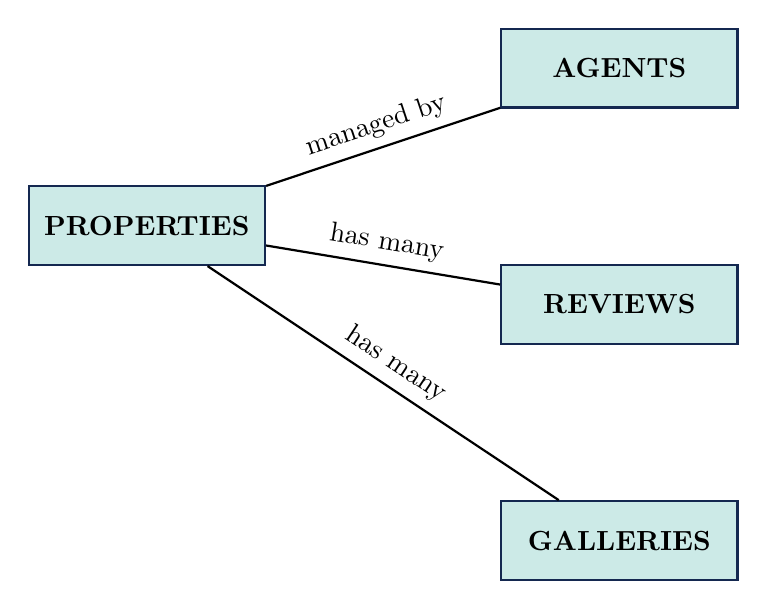
\begin{tikzpicture}[
    entity/.style={rectangle, draw=primarynavy, thick, fill=accentteal!20, minimum width=3cm, minimum height=1cm},
    relationship/.style={diamond, draw=accentorange, thick, fill=accentorange!20, aspect=2}
]

% Entities
\node[entity] (prop) at (0,0) {\textbf{PROPERTIES}};
\node[entity] (agent) at (6,2) {\textbf{AGENTS}};
\node[entity] (review) at (6,-1) {\textbf{REVIEWS}};
\node[entity] (gallery) at (6,-4) {\textbf{GALLERIES}};

% Relationships
\draw[thick, -] (prop) -- node[above, sloped] {managed by} (agent);
\draw[thick, -] (prop) -- node[above, sloped] {has many} (review);
\draw[thick, -] (prop) -- node[above, sloped] {has many} (gallery);

\end{tikzpicture}
\caption{Database Entity Relationship Diagram}
\end{figure}

\section{Properties Collection}

\begin{table}[h]
\small
\centering
\begin{tabularx}{\textwidth}{l l X c}
\toprule
\textbf{Field} & \textbf{Type} & \textbf{Description} & \textbf{Required} \\
\midrule
name & String & Property name & Yes \\
type & String & Property type (House, Villa, etc.) & Yes \\
description & Text & Detailed description & Yes \\
address & String & Physical address & Yes \\
geolocation & String & Lat/Long coordinates & No \\
price & Number & Property price & Yes \\
area & Number & Area in square feet & Yes \\
bedrooms & Number & Number of bedrooms & Yes \\
bathrooms & Number & Number of bathrooms & Yes \\
rating & Number & Average rating (1-5) & Yes \\
facilities & Array & List of amenities & No \\
image & String & Main property image URL & Yes \\
agent & Relationship & Related agent ID & Yes \\
reviews & Relationship & Array of review IDs & No \\
gallery & Relationship & Array of gallery IDs & No \\
\bottomrule
\end{tabularx}
\caption{Properties Collection Schema}
\end{table}

\section{Additional Collections}

\begin{definitionbox}
\textbf{Agents Collection:} Stores agent information including name, email, and avatar.

\textbf{Reviews Collection:} Contains user reviews with name, avatar, review text, and rating.

\textbf{Galleries Collection:} Stores additional property images for gallery view.
\end{definitionbox}

% ============================================
% CHAPTER 7: INSTALLATION & SETUP
% ============================================
\chapter{Installation \& Setup}

\section{Prerequisites}

Before starting, ensure you have the following installed:

\begin{itemize}
    \item \textbf{Node.js} (v18 or higher)
    \item \textbf{npm} or \textbf{yarn} package manager
    \item \textbf{Git} version control
    \item \textbf{Expo Go} app on your mobile device
\end{itemize}

\section{Installation Steps}

\subsection{Step 1: Clone Repository}

\begin{lstlisting}[language=bash]
git clone https://github.com/Mausam5055/Real-Estate-APP.git
cd Real-Estate-APP
\end{lstlisting}

\subsection{Step 2: Install Dependencies}

\begin{lstlisting}[language=bash]
npm install
# or
yarn install
\end{lstlisting}

\subsection{Step 3: Configure Environment Variables}

Create a \texttt{.env.local} file in the root directory:

\begin{lstlisting}[language=bash]
EXPO_PUBLIC_APPWRITE_ENDPOINT=https://cloud.appwrite.io/v1
EXPO_PUBLIC_APPWRITE_PROJECT_ID=your_project_id
EXPO_PUBLIC_APPWRITE_DATABASE_ID=your_database_id
EXPO_PUBLIC_APPWRITE_GALLERIES_COLLECTION_ID=your_galleries_id
EXPO_PUBLIC_APPWRITE_REVIEWS_COLLECTION_ID=your_reviews_id
EXPO_PUBLIC_APPWRITE_AGENTS_COLLECTION_ID=your_agents_id
EXPO_PUBLIC_APPWRITE_PROPERTIES_COLLECTION_ID=your_properties_id
EXPO_PUBLIC_APPWRITE_BUCKET_ID=your_bucket_id
\end{lstlisting}

\subsection{Step 4: Start Development Server}

\begin{lstlisting}[language=bash]
npm start
# or
npx expo start
\end{lstlisting}

\section{Appwrite Configuration}

\begin{enumerate}
    \item Create an account at \url{https://cloud.appwrite.io/}
    \item Create a new project
    \item Set up collections (Properties, Agents, Reviews, Galleries)
    \item Enable Google OAuth provider
    \item Copy credentials to \texttt{.env.local} file
\end{enumerate}

\begin{notebox}
\textbf{Database Seeding:} After setup, use the built-in seeding utility to populate your database with sample data. Access this feature from the Profile section in the app.
\end{notebox}

% ============================================
% CHAPTER 8: PROJECT STRUCTURE
% ============================================
\chapter{Project Structure}

\section{Directory Organization}

\begin{lstlisting}[language=bash, caption=Project Directory Structure]
Real-Estate-APP/
├── app/                          # Application screens
│   ├── (root)/                   # Protected routes
│   │   ├── (tabs)/              # Bottom tab navigation
│   │   │   ├── index.tsx        # Home screen
│   │   │   ├── explore.tsx      # Explore screen
│   │   │   └── profile.tsx      # Profile screen
│   │   └── properties/          # Property details
│   │       └── [id].tsx         # Dynamic detail page
│   ├── _layout.tsx              # Root layout
│   ├── sign-in.tsx              # Auth screen
│   └── seed-data.tsx            # DB seeding utility
├── assets/                       # Static assets
│   ├── fonts/                   # Custom fonts
│   ├── icons/                   # Icon images
│   └── images/                  # App images
├── components/                   # Reusable components
│   ├── Cards.tsx                # Property cards
│   ├── Comment.tsx              # Review comments
│   ├── Filters.tsx              # Filter component
│   ├── NoResults.tsx            # Empty state
│   └── Search.tsx               # Search bar
├── constants/                    # App constants
│   ├── icons.ts                 # Icon exports
│   ├── images.ts                # Image exports
│   └── data.ts                  # Static data
├── lib/                         # Core utilities
│   ├── appwrite.ts              # Appwrite config
│   ├── global-provider.tsx      # Global state
│   ├── useAppwrite.ts           # Data hook
│   ├── seed.ts                  # Seeding logic
│   └── data.ts                  # Sample data
├── .env.local                   # Environment vars
├── app.json                     # Expo config
├── package.json                 # Dependencies
├── tailwind.config.js           # Tailwind config
└── tsconfig.json                # TypeScript config
\end{lstlisting}

\section{Component Architecture}

\begin{keypoint}
The application follows a \textbf{modular component architecture} where each component is responsible for a single functionality. This promotes code reusability and maintainability.
\end{keypoint}

% ============================================
% CHAPTER 9: FUTURE ROADMAP
% ============================================
\chapter{Future Roadmap}

\section{Phase 1: Enhanced User Experience (Q1 2025)}

\begin{itemize}
    \item \textbf{Favorites/Wishlist Feature}
    \begin{itemize}
        \item Save properties for later viewing
        \item Sync across devices
        \item Share wishlist with others
    \end{itemize}
    
    \item \textbf{Advanced Filters}
    \begin{itemize}
        \item Price range slider
        \item Multiple facility selection
        \item Sort by distance, price, rating
    \end{itemize}
    
    \item \textbf{Property Comparison}
    \begin{itemize}
        \item Compare up to 3 properties side-by-side
        \item Visual comparison charts
        \item Export comparison as PDF
    \end{itemize}
\end{itemize}

\section{Phase 2: Engagement \& Notifications (Q2 2025)}

\begin{itemize}
    \item \textbf{Push Notifications}
    \begin{itemize}
        \item New property alerts based on preferences
        \item Price drop notifications
        \item Saved search alerts
    \end{itemize}
    
    \item \textbf{In-App Messaging}
    \begin{itemize}
        \item Direct chat with agents
        \item Schedule property viewings
        \item Real-time message notifications
    \end{itemize}
    
    \item \textbf{Virtual Tours}
    \begin{itemize}
        \item 360° property views
        \item Video walkthroughs
        \item AR room visualization
    \end{itemize}
\end{itemize}

\section{Phase 3: Advanced Features (Q3 2025)}

\begin{itemize}
    \item \textbf{AI-Powered Recommendations}
    \begin{itemize}
        \item Personalized property suggestions
        \item Smart search based on user behavior
        \item Price prediction models
    \end{itemize}
    
    \item \textbf{Mortgage Calculator}
    \begin{itemize}
        \item EMI calculator
        \item Loan eligibility checker
        \item Bank comparison
    \end{itemize}
    
    \item \textbf{Offline Mode}
    \begin{itemize}
        \item Cache property data for offline viewing
        \item Sync when back online
        \item Download property brochures
    \end{itemize}
\end{itemize}

\section{Phase 4: Social \& Integration (Q4 2025)}

\begin{itemize}
    \item Social media sharing
    \item Community reviews and ratings
    \item Google Maps integration
    \item Calendar integration for appointments
    \item Analytics dashboard
\end{itemize}

\section{Long-Term Vision}

\begin{table}[h]
\centering
\begin{tabularx}{\textwidth}{l X}
\toprule
\textbf{Feature} & \textbf{Description} \\
\midrule
Multi-Language Support & Add support for regional languages \\
Dark Mode & Complete dark theme implementation \\
Web Platform & Expand to web using React.js \\
Admin Dashboard & Property management portal for agents \\
Payment Gateway & Integrate booking/token payment \\
Blockchain Integration & Property ownership verification using NFTs \\
\bottomrule
\end{tabularx}
\caption{Long-Term Vision}
\end{table}

% ============================================
% CHAPTER 10: WORKFLOW DIAGRAM
% ============================================
\chapter{Application Workflow}

\section{User Journey Flowchart}

\begin{figure}[h]
\centering
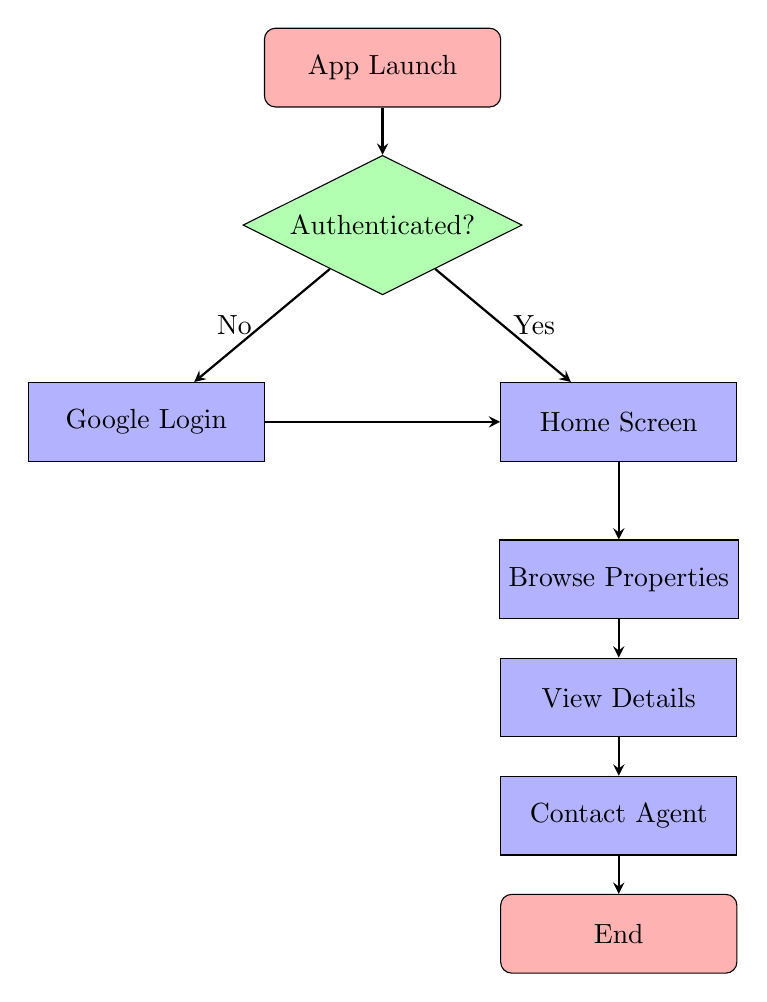
\begin{tikzpicture}[
    node distance=1.5cm,
    startstop/.style={rectangle, rounded corners, minimum width=3cm, minimum height=1cm, text centered, draw=black, fill=red!30},
    process/.style={rectangle, minimum width=3cm, minimum height=1cm, text centered, draw=black, fill=blue!30},
    decision/.style={diamond, minimum width=3cm, minimum height=1cm, text centered, draw=black, fill=green!30, aspect=2},
    arrow/.style={->, >=stealth, thick}
]

\node[startstop] (start) {App Launch};
\node[decision, below of=start, yshift=-0.5cm] (auth) {Authenticated?};
\node[process, below of=auth, yshift=-1cm, xshift=-3cm] (login) {Google Login};
\node[process, below of=auth, yshift=-1cm, xshift=3cm] (home) {Home Screen};
\node[process, below of=home, yshift=-0.5cm] (browse) {Browse Properties};
\node[process, below of=browse] (details) {View Details};
\node[process, below of=details] (contact) {Contact Agent};
\node[startstop, below of=contact] (end) {End};

\draw[arrow] (start) -- (auth);
\draw[arrow] (auth) -- node[left] {No} (login);
\draw[arrow] (auth) -- node[right] {Yes} (home);
\draw[arrow] (login) -- (home);
\draw[arrow] (home) -- (browse);
\draw[arrow] (browse) -- (details);
\draw[arrow] (details) -- (contact);
\draw[arrow] (contact) -- (end);

\end{tikzpicture}
\caption{User Journey Flowchart}
\end{figure}

\section{Data Flow Pipeline}

\begin{figure}[h]
\centering
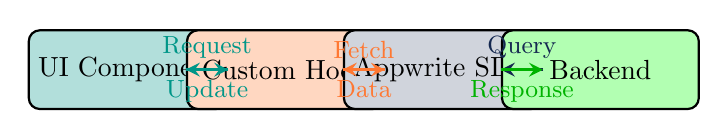
\begin{tikzpicture}[
    node distance=2cm,
    box/.style={rectangle, rounded corners, minimum width=2.5cm, minimum height=1cm, text centered, draw=black, thick},
    arrow/.style={->, >=stealth, very thick}
]

\node[box, fill=accentteal!30] (ui) {UI Component};
\node[box, fill=accentorange!30, right of=ui] (hook) {Custom Hook};
\node[box, fill=primarynavy!20, right of=hook] (sdk) {Appwrite SDK};
\node[box, fill=green!30, right of=sdk] (backend) {Backend};

\draw[arrow, accentteal] (ui) -- node[above, font=\small] {Request} (hook);
\draw[arrow, accentorange] (hook) -- node[above, font=\small] {Fetch} (sdk);
\draw[arrow, primarynavy] (sdk) -- node[above, font=\small] {Query} (backend);
\draw[arrow, green!70!black] (backend) -- node[below, font=\small] {Response} (sdk);
\draw[arrow, accentorange] (sdk) -- node[below, font=\small] {Data} (hook);
\draw[arrow, accentteal] (hook) -- node[below, font=\small] {Update} (ui);

\end{tikzpicture}
\caption{Data Flow Pipeline}
\end{figure}

% ============================================
% CHAPTER 11: ADVANTAGES
% ============================================
\chapter{Advantages \& Benefits}

\section{Technical Advantages}

\begin{enumerate}
    \item \textbf{Cross-Platform Development}
    \begin{itemize}
        \item Single codebase for iOS and Android
        \item Reduced development time and cost
        \item Consistent user experience across platforms
    \end{itemize}
    
    \item \textbf{Type Safety with TypeScript}
    \begin{itemize}
        \item Catch errors during development
        \item Better IDE support and autocomplete
        \item Improved code maintainability
    \end{itemize}
    
    \item \textbf{Backend-as-a-Service}
    \begin{itemize}
        \item No backend infrastructure management
        \item Built-in authentication and database
        \item Automatic scaling and security
    \end{itemize}
    
    \item \textbf{Modern UI Framework}
    \begin{itemize}
        \item Rapid UI development with NativeWind
        \item Consistent design system
        \item Responsive layouts
    \end{itemize}
\end{enumerate}

\section{Business Advantages}

\begin{keypoint}
Real Scout provides significant business value through:
\begin{itemize}
    \item Faster time-to-market
    \item Lower development costs
    \item Scalable architecture
    \item Easy maintenance and updates
    \item Rich feature set out of the box
\end{itemize}
\end{keypoint}

\section{User Experience Benefits}

\begin{table}[h]
\centering
\begin{tabularx}{\textwidth}{l X}
\toprule
\textbf{Benefit} & \textbf{Impact} \\
\midrule
Fast Performance & Quick property browsing and search \\
Intuitive UI & Easy navigation for all user types \\
Secure Login & Peace of mind with Google OAuth \\
Rich Information & Comprehensive property details \\
Visual Gallery & High-quality property images \\
Agent Profiles & Direct communication with agents \\
\bottomrule
\end{tabularx}
\caption{User Experience Benefits}
\end{table}

% ============================================
% CHAPTER 12: CONCLUSION
% ============================================
\chapter{Conclusion}

\section{Summary}

Real Scout represents a modern approach to real estate mobile applications, combining cutting-edge technologies with user-centric design. The application successfully demonstrates:

\begin{itemize}
    \item Effective use of React Native for cross-platform development
    \item Seamless integration with Appwrite backend services
    \item Secure authentication through Google OAuth
    \item Scalable and maintainable code architecture
    \item Rich feature set for property browsing and exploration
\end{itemize}

\section{Key Takeaways}

\begin{definitionbox}
\textbf{React Native + Appwrite:} This combination provides a powerful stack for rapid mobile app development with minimal backend management.

\textbf{TypeScript:} Adds type safety and improves developer experience significantly.

\textbf{NativeWind:} Brings the productivity of Tailwind CSS to React Native development.
\end{definitionbox}

\section{Future Outlook}

The roadmap for Real Scout includes exciting features such as AI-powered recommendations, virtual tours, and blockchain integration. These enhancements will further solidify its position as a comprehensive real estate solution.

\begin{notebox}
This project serves as an excellent foundation for anyone looking to build production-ready mobile applications using modern technologies and best practices.
\end{notebox}

% ============================================
% APPENDICES
% ============================================
\appendix

\chapter{Additional Resources}

\section{Useful Links}

\begin{itemize}
    \item GitHub Repository: \url{https://github.com/Mausam5055/Real-Estate-APP}
    \item React Native Documentation: \url{https://reactnative.dev/}
    \item Expo Documentation: \url{https://docs.expo.dev/}
    \item Appwrite Documentation: \url{https://appwrite.io/docs}
    \item NativeWind Documentation: \url{https://www.nativewind.dev/}
\end{itemize}

\section{License Information}

This project is licensed under the MIT License. Copyright (c) 2024 Mausam Kar.

\vspace{1cm}

\begin{center}
\Large\textbf{Thank you for reading!}

\vspace{0.5cm}

\textit{For questions or contributions, please visit the GitHub repository.}
\end{center}

\end{document}
